%%%%%%%%%%%%%%%%%%%%%%%%%%%%%%%%%%%%%%%%%%%%%%%%%%%%%%%%%%%%%%%%%%%%%%%
% Ansys Techcon 2022 - PyVista – Visualizing CAE and Results with Python
%%%%%%%%%%%%%%%%%%%%%%%%%%%%%%%%%%%%%%%%%%%%%%%%%%%%%%%%%%%%%%%%%%%%%%%
\documentclass[t]{beamer}

\usetheme{Ansys2022}

\usepackage{animate}
\usepackage{svg}
\usepackage{bbding,pifont}
\usepackage{minted}
\usepackage{xcolor}
\usepackage{pdfpages}
\usepackage{listings}
\usepackage{hyperref}

\usepackage{tikz}
\usetikzlibrary{intersections}
\usetikzlibrary{shapes.geometric, arrows,positioning}

\usepackage[edges]{forest}
\hypersetup{
    colorlinks=true,
    linkcolor=blue,
    filecolor=magenta,
    urlcolor=cyan,
}


\urlstyle{same}
\setbeamercolor{background canvas}{bg=}

\definecolor{bleudefrance}{rgb}{0.19, 0.55, 0.91}

%%%%%%%%%%%%%%%%%%%%%%%%%%%%%%%%%%%%%%%%%%%%%%%%%%%%%%%%%%%%%%%%%%%%%%%%%%%%%%%

\tikzset{
  startstop/.style={
    rectangle,
    rounded corners,
    minimum width=3cm,
    minimum height=0.75cm,
    align=center,
    draw=black,
    fill=ANSYS@Gold,
    },
  process/.style={
    rectangle,
    minimum width=3cm,
    minimum height=0.75cm,
    align=center,
    draw=black,
    fill=ANSYS@Blue,
    text=white,
    },
  decision/.style={
    diamond,
    aspect=4,
    minimum width=3cm,
    minimum height=1cm,
    align=center,
    draw=black,
    fill=ANSYS@Blue,
    text=white,
    },
  arrow/.style={thick,->,>=stealth},
  dec/.style={
    ellipse,
    align=center,
    draw=black,
    fill=ANSYS@Bronze,
    },
}

\begin{document}

%%%%%%%%%%%%%%%%%%%%%%%%%%%%%%%%%%%%%%%%%%%%%%%%%%%%%%%%%%%%%%%%%%%%%%%%%%%%%%%
%% Title Slide

\title{PyVista \\
  Visualizing CAE Results with Python}
%% \subtitle{}
\author{Alex Kaszynski}
\date{\today}

\titleframe{}


%%%%%%%%%%%%%%%%%%%%%%%%%%%%%%%%%%%%%%%%%%%%%%%%%%%%%%%%%%%%%%%%%%%%%%%%%%%%%%%
%% Table of contents

\begin{frame}{Table of Contents}
  \tableofcontents
  \vspace{200pt}  %% force top tight
\end{frame}

%%%%%%%%%%%%%%%%%%%%%%%%%%%%%%%%%%%%%%%%%%%%%%%%%%%%%%%%%%%%%%%%%%%%%%%%%%%%%%%
\section{PyVista - Introduction}

%%%%%%%%%%%%%%%%%%%%%%%%%%%%%%%%%%%%%%%%%%%%%%%%%%%%%%%%%%%%%%%%%%%%%%%%%%%%%%%
\begin{frame}
  \frametitle{PyVista - Introduction}

  \begin{columns}[T]

    \begin{column}{.5\textwidth}
      \vspace{-10pt}
      \inputminted[fontsize=\footnotesize]{python}{code/pv_example1.py}
    \end{column}

    \begin{column}{.4\textwidth}
      \vspace{-20pt}
      \centering
      
\includegraphics[height=0.2\textheight]{figures/pyvista_logo.png}
    \end{column}

  \end{columns}
  \vspace{5pt}

  PyVista allows you to rapidly load meshes and handles much of the “grunt
  work” of setting up plots, connecting classes and pipelines, and cleaning up
  plotting windows.

  \vspace{5pt}

  \begin{exampleblock}{PyVista allows you to:}
    \begin{itemize}
    \item Easily load a wide variety of datasets and file types.
    \item Leverage powerful VTK filters and perform complex data operations.
    \item Quickly set up simple or complex plots.
    \end{itemize}
  \end{exampleblock}

\end{frame}


%%%%%%%%%%%%%%%%%%%%%%%%%%%%%%%%%%%%%%%%%%%%%%%%%%%%%%%%%%%%%%%%%%%%%%%%%%%%%%%
\begin{frame}
  \frametitle{PyVista - Popularity and Growth}

  \vspace{-15pt}

  \begin{center}
    \begin{columns}[T]
      \begin{column}{.5\textwidth}
        \small
        \begin{itemize}
          \item Already the most popular 3d visualization library on PyPI.
          \item Designed not just for visualization, but for scientific
            visualization focused on data post-processing, file IO, and
            interoperability with other libraries.
        \end{itemize}
        \vspace{10pt}
        \href{https://pyviz.org/tools.html}{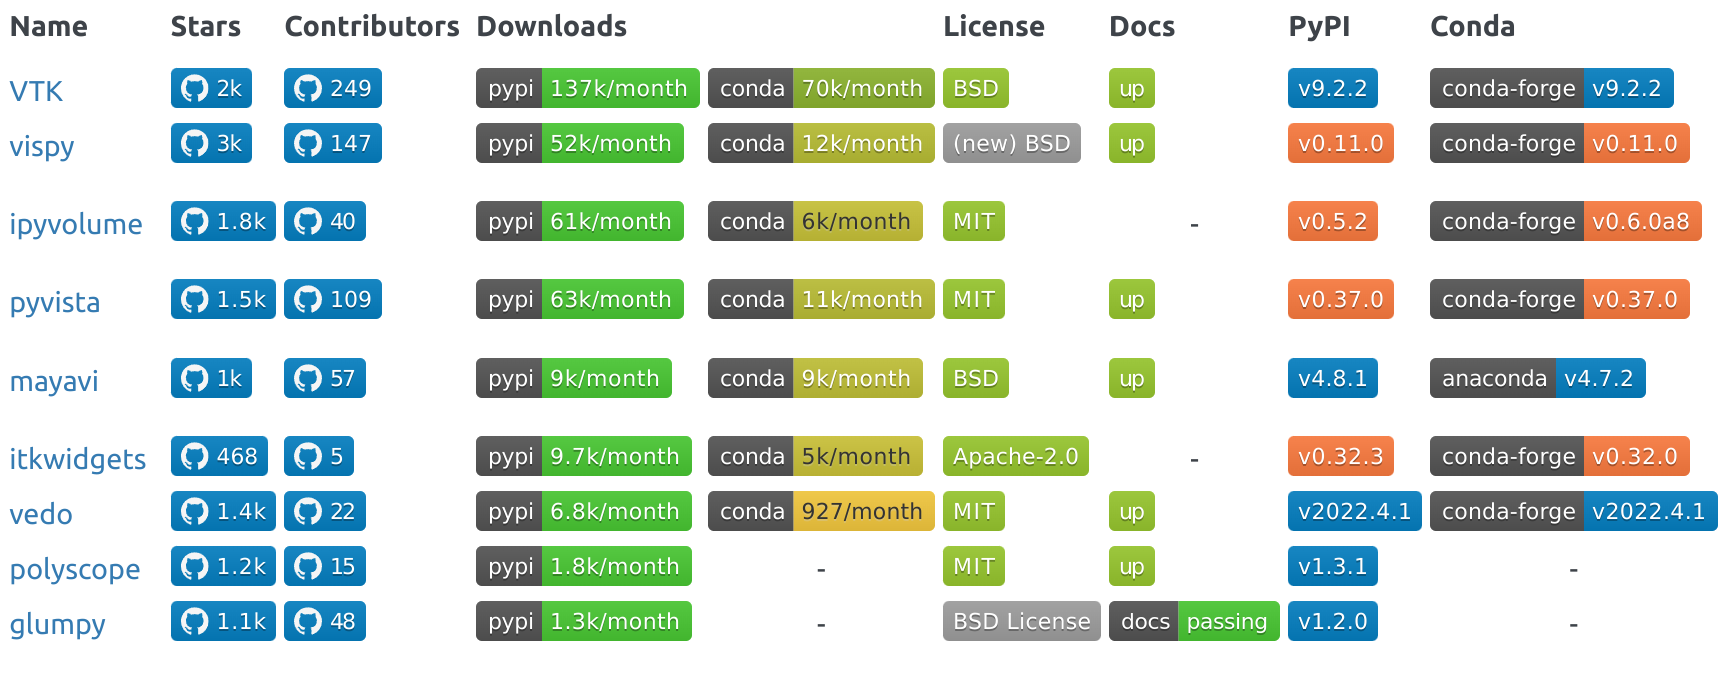
\includegraphics[width=1.1\textwidth]{figures/overview_sciviz.png}}
      \end{column}

      \begin{column}{.5\textwidth}
        \vspace{-5pt}
        \centering
        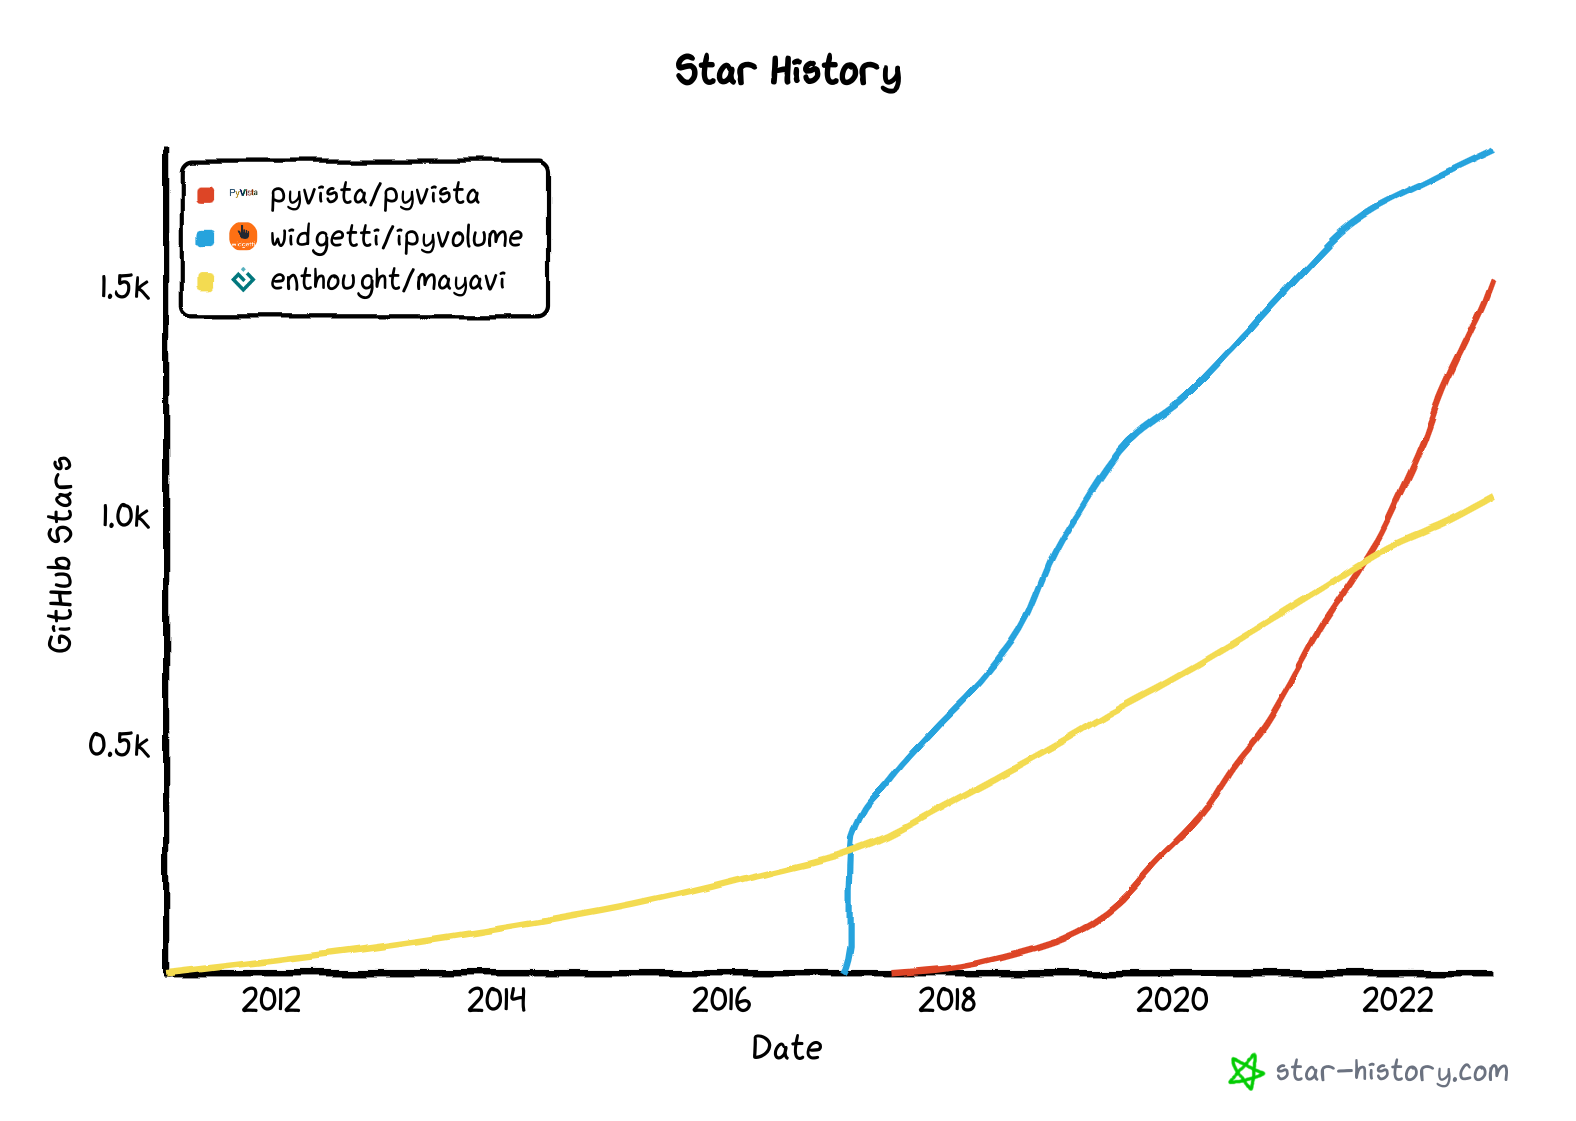
\includegraphics[width=0.9\textwidth]{figures/overview-graph.png}
      \end{column}
    \end{columns}
  \end{center}  

\end{frame}


%%%%%%%%%%%%%%%%%%%%%%%%%%%%%%%%%%%%%%%%%%%%%%%%%%%%%%%%%%%%%%%%%%%%%%%%%%%%%%%
\subsection{Where is it already used?}
\begin{frame}
  \frametitle{PyVista - Current Usage}

  \vspace{-8pt}
  PyVista is already being used by:
  \vspace{-8pt}

  \begin{columns}[T]
    \begin{column}{.3\textwidth}
        \begin{exampleblock}{ACE \& Partners}
        \inputminted[fontsize=\tiny]{python}{code/dpf_simple.py}
        \centering
        \href{https://www.padtinc.com/2022/07/18/ansys-scripting-python-p1-solve-post/}{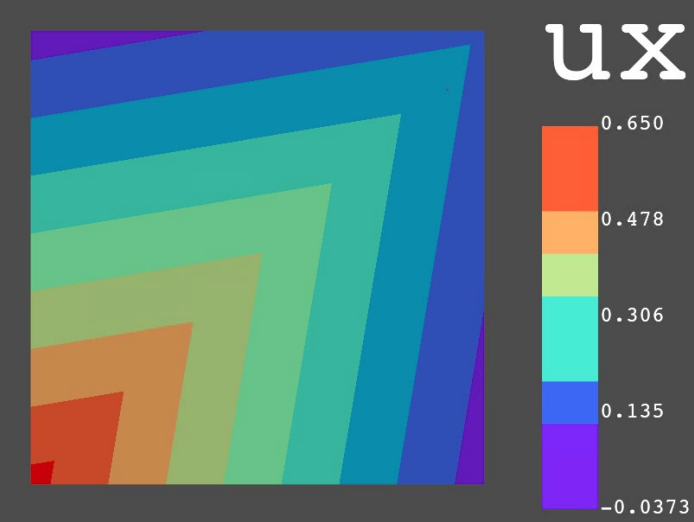
\includegraphics[width=0.95\textwidth]{figures/dpf_simple.png}}
        \end{exampleblock}
      \end{column}

    \begin{column}{.3\textwidth}
        \begin{exampleblock}{PyAnsys}
        \inputminted[fontsize=\tiny]{python}{code/pymapdl_eo_disc.py}
        \centering
        \href{https://github.com/pyansys/ray-segments-pyvista}{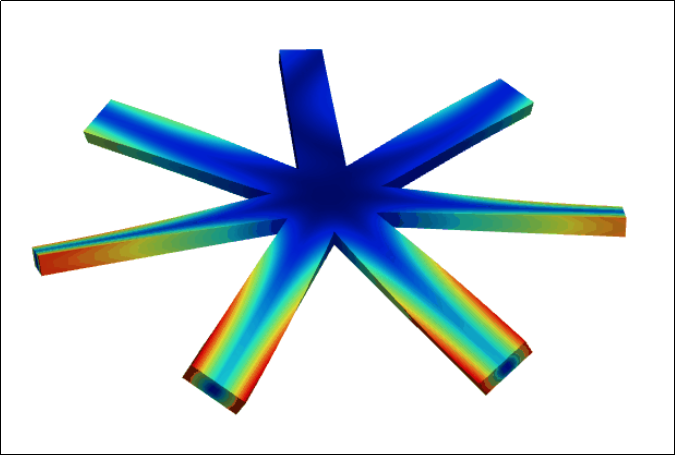
\includegraphics[width=0.95\textwidth]{figures/pymapdl_eo_disc.png}}
        \end{exampleblock}
      \end{column}

    \begin{column}{.3\textwidth}
        \begin{exampleblock}{OnScale}
        \inputminted[fontsize=\tiny]{python}{code/onscale_pyvista.py}
        \centering
        \href{https://github.com/pyansys/ray-segments-pyvista}{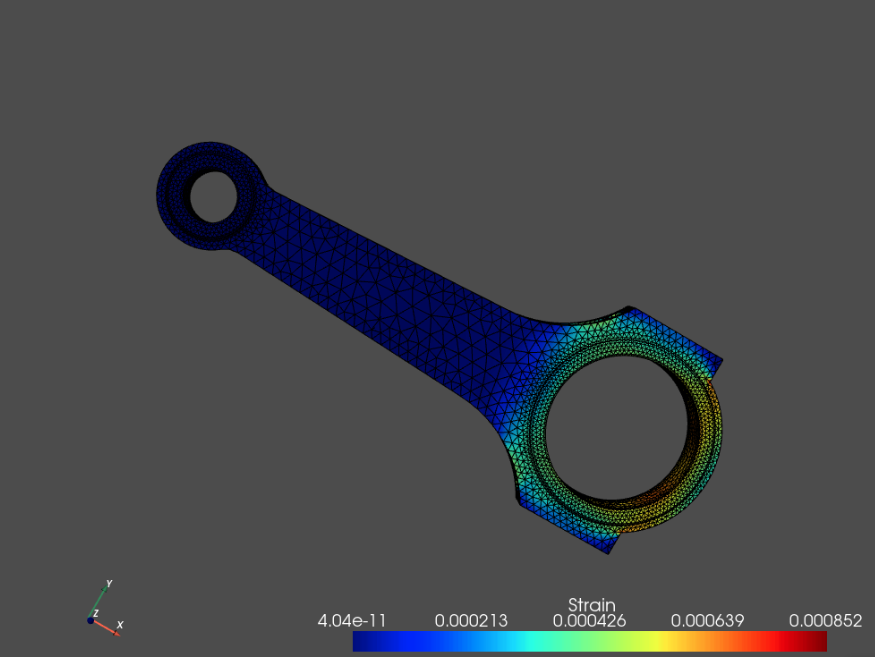
\includegraphics[width=0.95\textwidth]{figures/onscale_pyvista.png}}
        \end{exampleblock}
      \end{column}

  \end{columns}

\end{frame}

%%%%%%%%%%%%%%%%%%%%%%%%%%%%%%%%%%%%%%%%%%%%%%%%%%%%%%%%%%%%%%%%%%%%%%%%%%%%%%%
\subsection{Quick Example}
\begin{frame}
  \frametitle{Quick Example - Path Operation}

  \begin{columns}[T]
    \begin{column}{.5\textwidth}
      \vspace{-15pt}
      \inputminted[fontsize=\footnotesize]{python}{code/path_op.py}
    \end{column}

    \begin{column}{.5\textwidth}
      \vspace{-15pt}
      \centering
      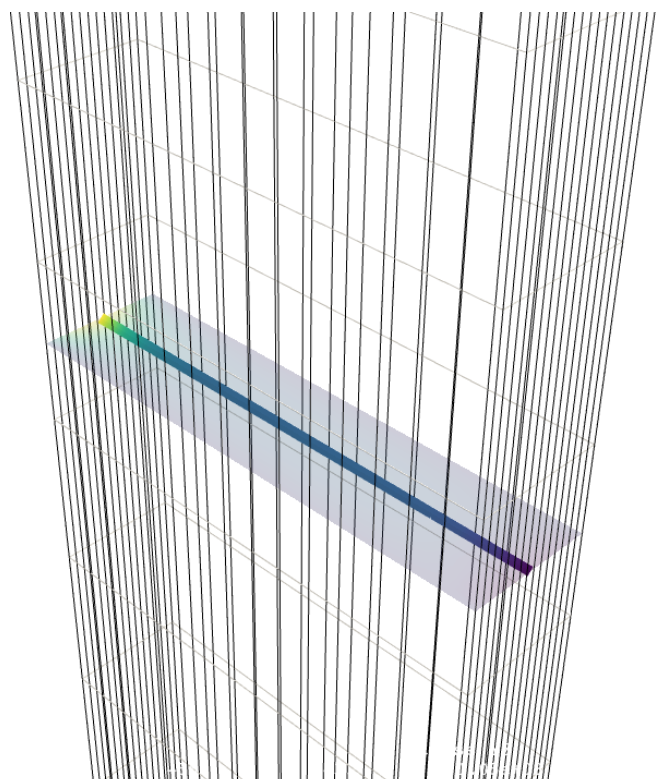
\includegraphics[width=0.75\textwidth]{figures/path_op.png}
    \end{column}
  \end{columns}

\end{frame}


%%%%%%%%%%%%%%%%%%%%%%%%%%%%%%%%%%%%%%%%%%%%%%%%%%%%%%%%%%%%%%%%%%%%%%%%%%%%%%%
\begin{frame}
  \frametitle{Quick Example - Path Operation vs PyMAPDL}

  \begin{columns}[T]
    \begin{column}{.5\textwidth}
      \vspace{-15pt}
      \inputminted[fontsize=\footnotesize]{python}{code/path_op_vs_pymapdl.py}
    \end{column}

    \begin{column}{.5\textwidth}
      \vspace{-15pt}
      \centering
      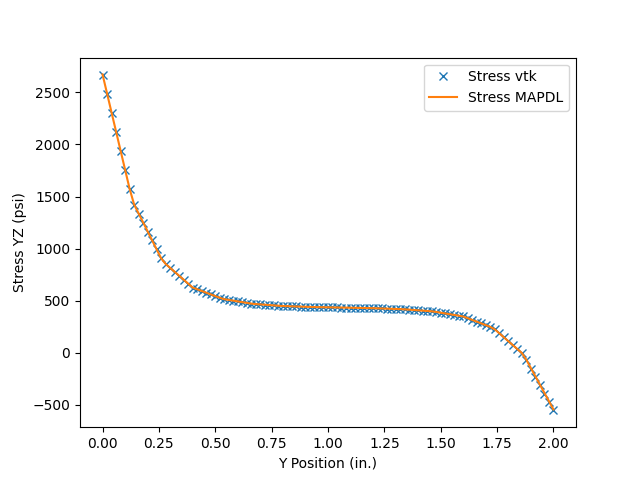
\includegraphics[width=1.0\textwidth]{figures/path_op_vs_pymapdl.png}
    \end{column}
  \end{columns}

\end{frame}


%%%%%%%%%%%%%%%%%%%%%%%%%%%%%%%%%%%%%%%%%%%%%%%%%%%%%%%%%%%%%%%%%%%%%%%%%%%%%%%
\subsection{Comparison - VTK vs. PyVista}
\begin{frame}
  \frametitle{Comparison - VTK vs. PyVista}
  \begin{columns}[T]
    \begin{column}{.5\textwidth}
      \vspace{-15pt}
      \inputminted[fontsize=\footnotesize]{python}{code/vtk_example.py}
    \end{column}

    \begin{column}{.5\textwidth}
      \vspace{-15pt}
      \inputminted[fontsize=\footnotesize]{python}{code/pv_example.py}
      \begin{center}
        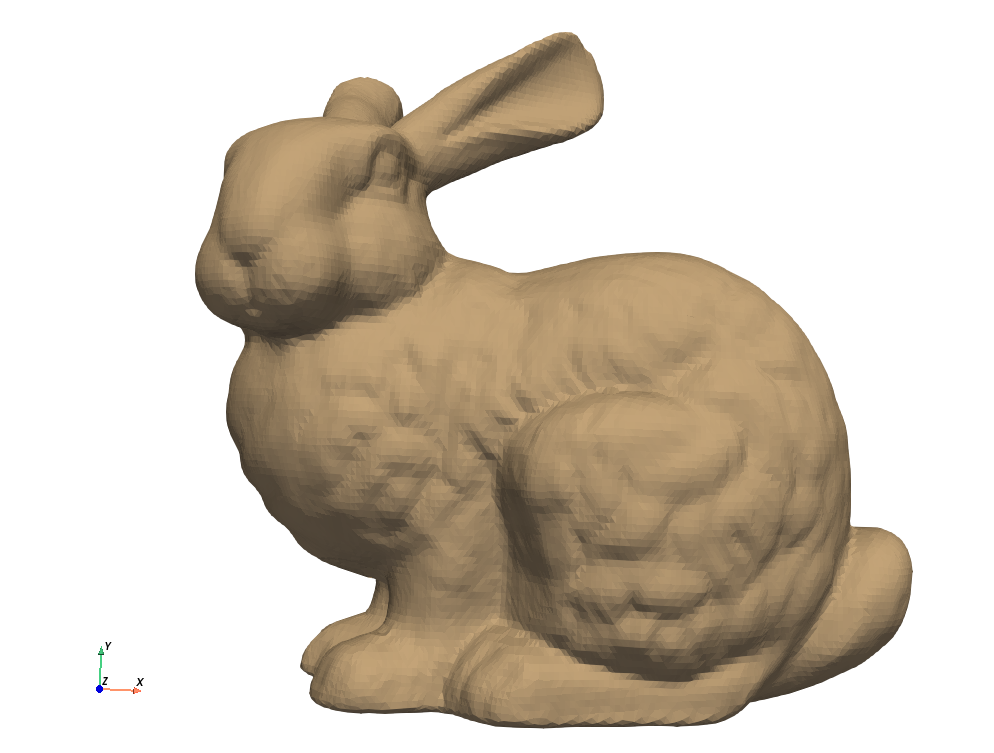
\includegraphics[width=0.9\textwidth]{figures/pv_example.png}
        \end{center}
    \end{column}
  \end{columns}

\end{frame}


%%%%%%%%%%%%%%%%%%%%%%%%%%%%%%%%%%%%%%%%%%%%%%%%%%%%%%%%%%%%%%%%%%%%%%%%%%%%%%%
\transitionframe{Getting Started}
\section{Getting Started}

\begin{frame}
  \frametitle{Getting Started}
  \tableofcontents[currentsection]
  \vspace{200pt}  %% force top tight
\end{frame}

%%%%%%%%%%%%%%%%%%%%%%%%%%%%%%%%%%%%%%%%%%%%%%%%%%%%%%%%%%%%%%%%%%%%%%%%%%%%%%%
\subsection{Installation}
\begin{frame}[fragile=singleslide]
  \frametitle{Installation}
  \vspace{-10pt}

  \begin{columns}[T]
    \begin{column}{.5\textwidth}
      \vspace{-10pt}
      \begin{exampleblock}{pip}
        \begin{lstlisting}[basicstyle=\ttfamily\footnotesize]
pip install pyvista
        \end{lstlisting}
      \end{exampleblock}

    \end{column}

    \begin{column}{.5\textwidth}
      \vspace{-10pt}
      \begin{exampleblock}{conda}
        \begin{lstlisting}[basicstyle=\ttfamily\footnotesize]
conda install -c conda-forge pyvista
        \end{lstlisting}
      \end{exampleblock}

    \end{column}
  \end{columns}

  \vspace{5pt}

  \centering
  \href{https://asciinema.org/a/507562}{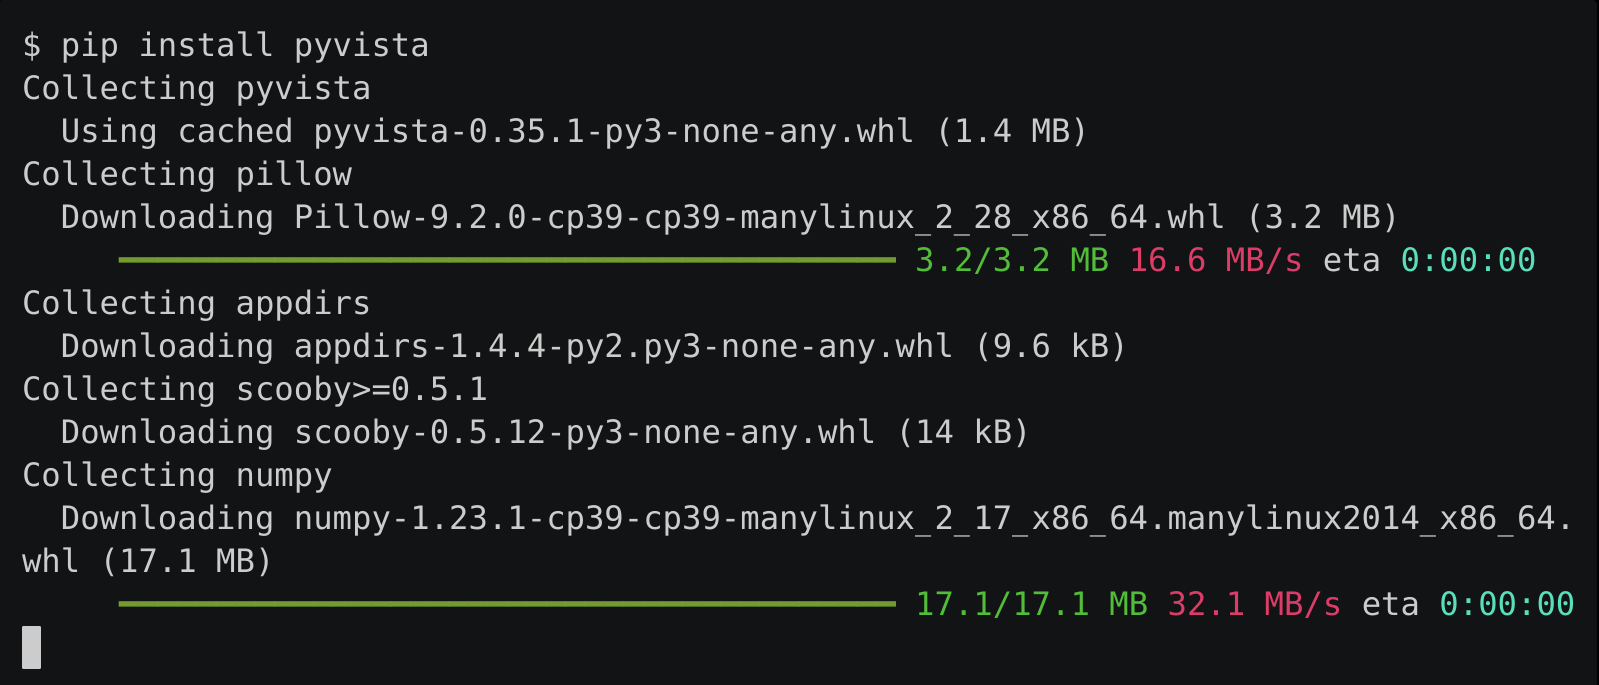
\includegraphics[width=0.76\textwidth]{figures/install_pyvista.png}}

\end{frame}


%%%%%%%%%%%%%%%%%%%%%%%%%%%%%%%%%%%%%%%%%%%%%%%%%%%%%%%%%%%%%%%%%%%%%%%%%%%%%%%
\transitionframe{Examples}
\section{Examples}

\begin{frame}
  \frametitle{Examples}
  \tableofcontents[currentsection]
  \vspace{200pt}  %% force top tight
\end{frame}

%%%%%%%%%%%%%%%%%%%%%%%%%%%%%%%%%%%%%%%%%%%%%%%%%%%%%%%%%%%%%%%%%%%%%%%%%%%%%%%
\subsection{Basic Plot}
\begin{frame}
  \frametitle{Examples - Basic Plot}

  \begin{center}
    \begin{columns}[T]
      \begin{column}{.5\textwidth}
        \inputminted[fontsize=\footnotesize]{python}{code/basic_usage.py}
      \end{column}

      \begin{column}{.5\textwidth}
        \centering
        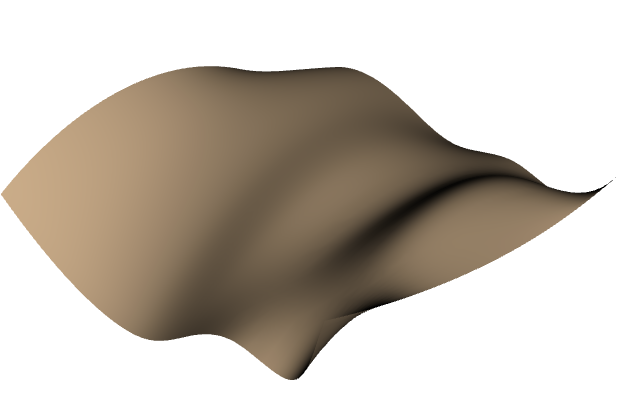
\includegraphics[width=1.0\textwidth]{figures/basic_usage.png}
      \end{column}
    \end{columns}
  \end{center}

\end{frame}


%%%%%%%%%%%%%%%%%%%%%%%%%%%%%%%%%%%%%%%%%%%%%%%%%%%%%%%%%%%%%%%%%%%%%%%%%%%%%%%
\subsection{Basic Volumetric Plot}
\begin{frame}
  \frametitle{Examples - Basic Volumetric Plot}

  \begin{center}
    \begin{columns}[T]
      \begin{column}{.5\textwidth}
        \inputminted[fontsize=\footnotesize]{python}{code/basic_usage2.py}
      \end{column}

      \begin{column}{.5\textwidth}
        \centering
        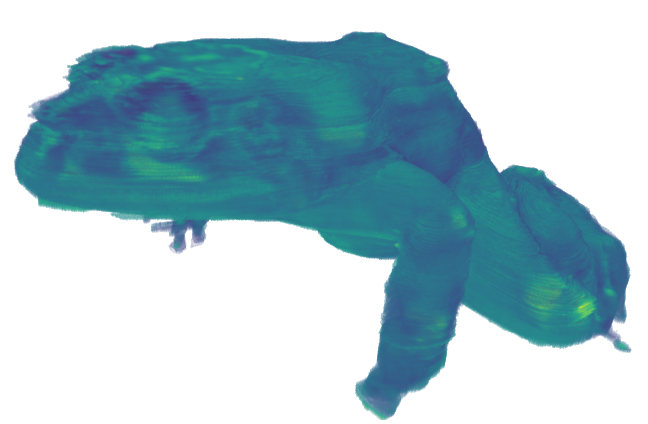
\includegraphics[width=1.0\textwidth]{figures/basic_usage2.png}
      \end{column}
    \end{columns}
  \end{center}

\end{frame}

%%%%%%%%%%%%%%%%%%%%%%%%%%%%%%%%%%%%%%%%%%%%%%%%%%%%%%%%%%%%%%%%%%%%%%%%%%%%%%%
\subsection{Filters}
\begin{frame}
  \frametitle{Examples - Filters}
  \vspace{-10pt}

  \begin{center}
    \begin{columns}[T]
      \begin{column}{.5\textwidth}
        \inputminted[fontsize=\footnotesize]{python}{code/filters.py}
      \end{column}

      \begin{column}{.5\textwidth}
        \centering
        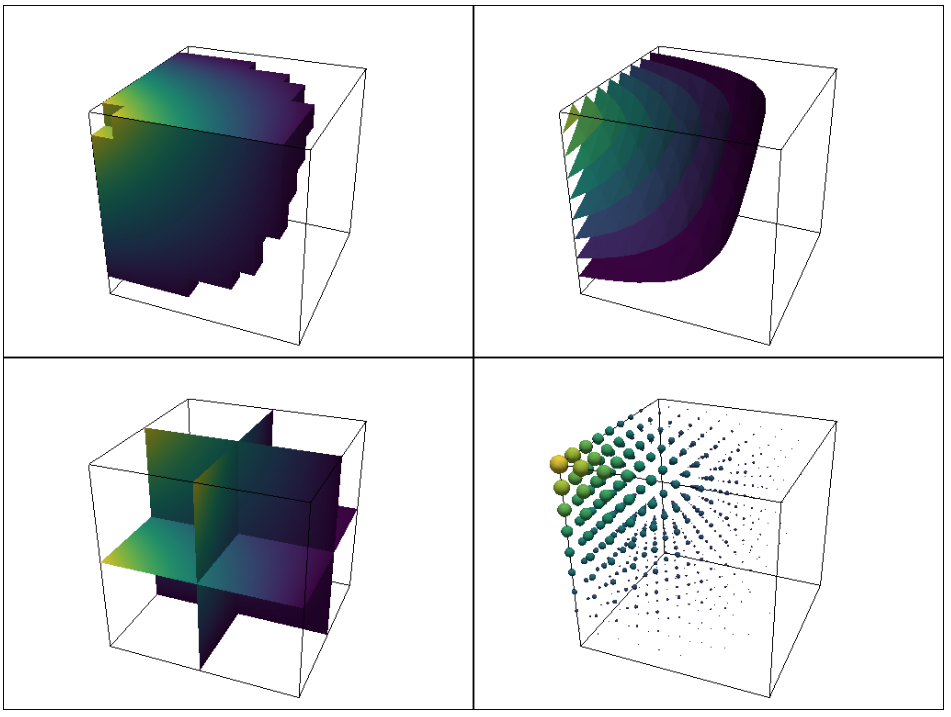
\includegraphics[width=1.0\textwidth]{figures/filters.png}
      \end{column}
    \end{columns}
  \end{center}

\end{frame}

%%%%%%%%%%%%%%%%%%%%%%%%%%%%%%%%%%%%%%%%%%%%%%%%%%%%%%%%%%%%%%%%%%%%%%%%%%%%%%%
\begin{frame}
  \frametitle{Examples - Widgets}

  \begin{center}
    \begin{columns}[T]
      \begin{column}{.5\textwidth}
        \inputminted[fontsize=\footnotesize]{python}{code/widgets_ex.py}
      \end{column}

      \begin{column}{.5\textwidth}
        \vspace{-25pt}
        \centering
        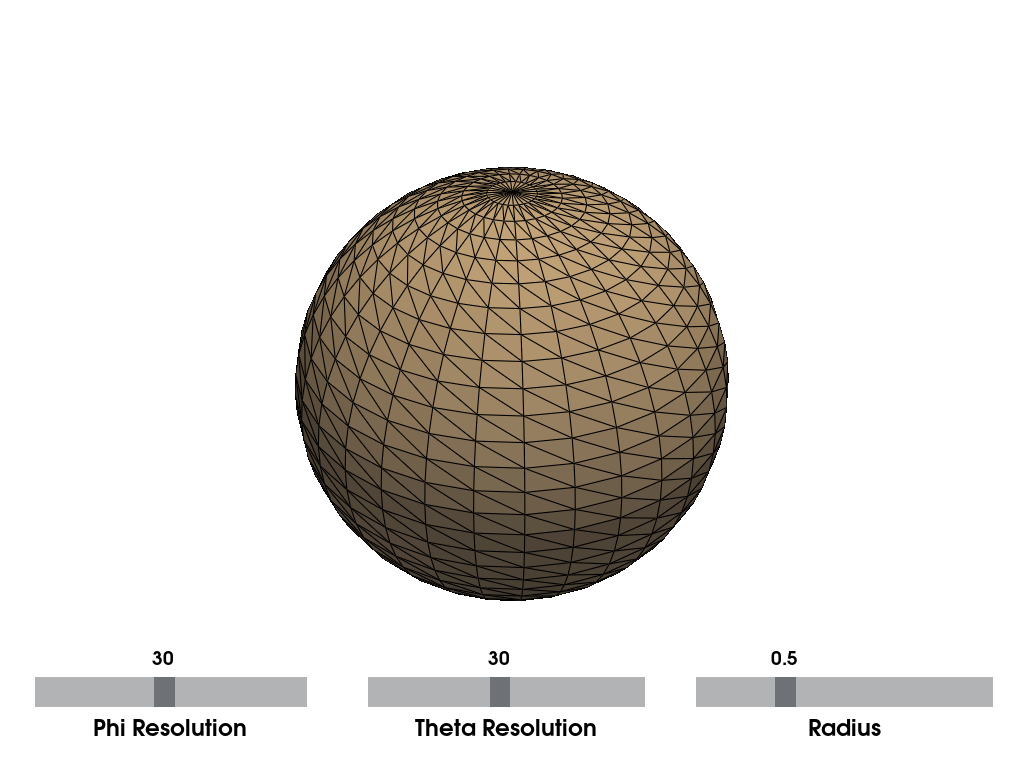
\includegraphics[width=1.0\textwidth]{figures/sphx_glr_d_multi-slider-widget_001}
      \end{column}
    \end{columns}
  \end{center}

\end{frame}

%%%%%%%%%%%%%%%%%%%%%%%%%%%%%%%%%%%%%%%%%%%%%%%%%%%%%%%%%%%%%%%%%%%%%%%%%%%%%%%
\subsection{PyInstaller and PyQT}
\begin{frame}
  \frametitle{Examples - PyInstaller and PyQT}

  \vspace{-15pt}

  \begin{center}
    \begin{columns}[T]
      \begin{column}{.5\textwidth}
        \small
        \begin{itemize}
          \item Use PyInstaller and PyQT or PySide to create a standalone application.
          \item Multi-platform. Build on the OS you intend to deploy.
          \item Compatible with GitHub Actions and can be automated.
          \item Deploy as using an installer like NSIS.
        \end{itemize}
        \vspace{5pt}
        \inputminted[fontsize=\footnotesize]{bash}{code/pyinstaller.py}
      \end{column}

      \begin{column}{.5\textwidth}
        %% \vspace{-25pt}
        \centering
        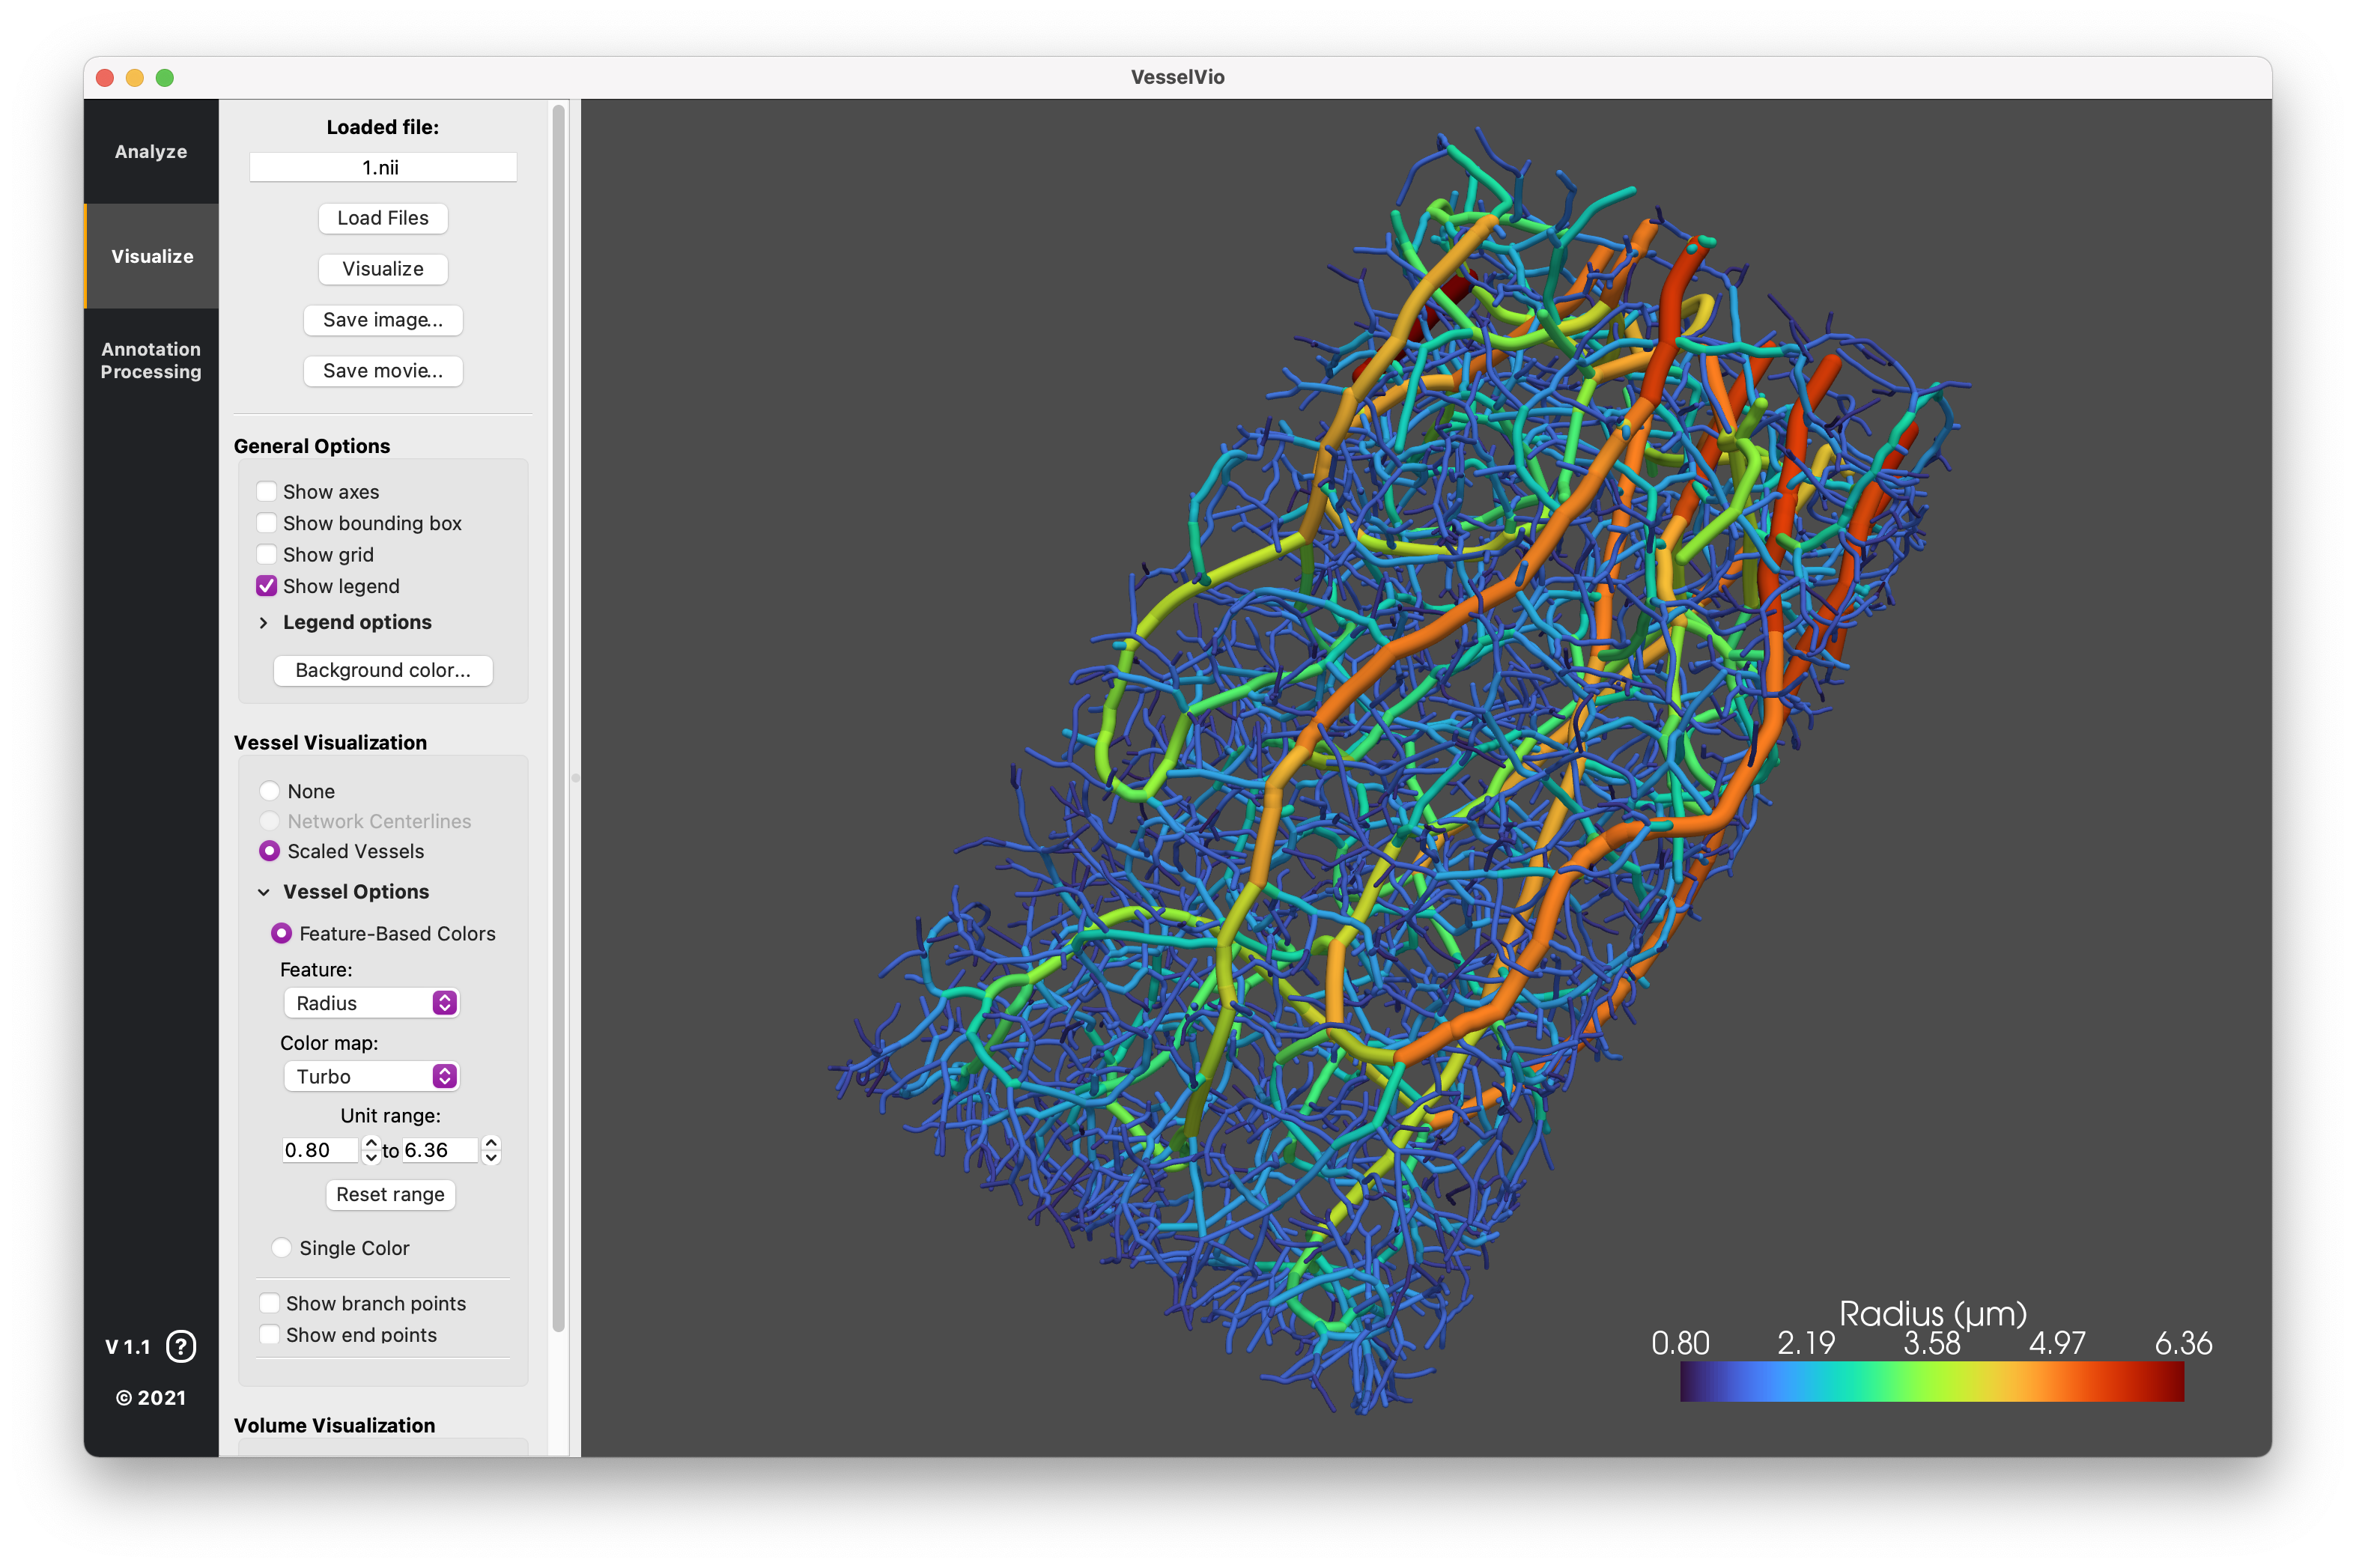
\includegraphics[width=1.0\textwidth]{figures/VesselVio.png}
      \end{column}
    \end{columns}
  \end{center}

\end{frame}


%%%%%%%%%%%%%%%%%%%%%%%%%%%%%%%%%%%%%%%%%%%%%%%%%%%%%%%%%%%%%%%%%%%%%%%%%%%%%%%
\begin{frame}
  \frametitle{Examples - Documentation with Sphinx}

  \vspace{-15pt}

  \begin{center}
    \begin{columns}[T]
      \begin{column}{.5\textwidth}
        \small
        \begin{itemize}
          \item PyVista supports the Sphinx documentation generator.
          \item Allows you to generate static and interactive documentation.
          \item Place code snippets directly in the documentation as examples.
        \end{itemize}
        \vspace{5pt}
        \inputminted[fontsize=\footnotesize]{bash}{code/sphinx_conf.py}
      \end{column}

      \begin{column}{.5\textwidth}
        \vspace{-5pt}
        \centering
        \href{https://docs.pyvista.org/}{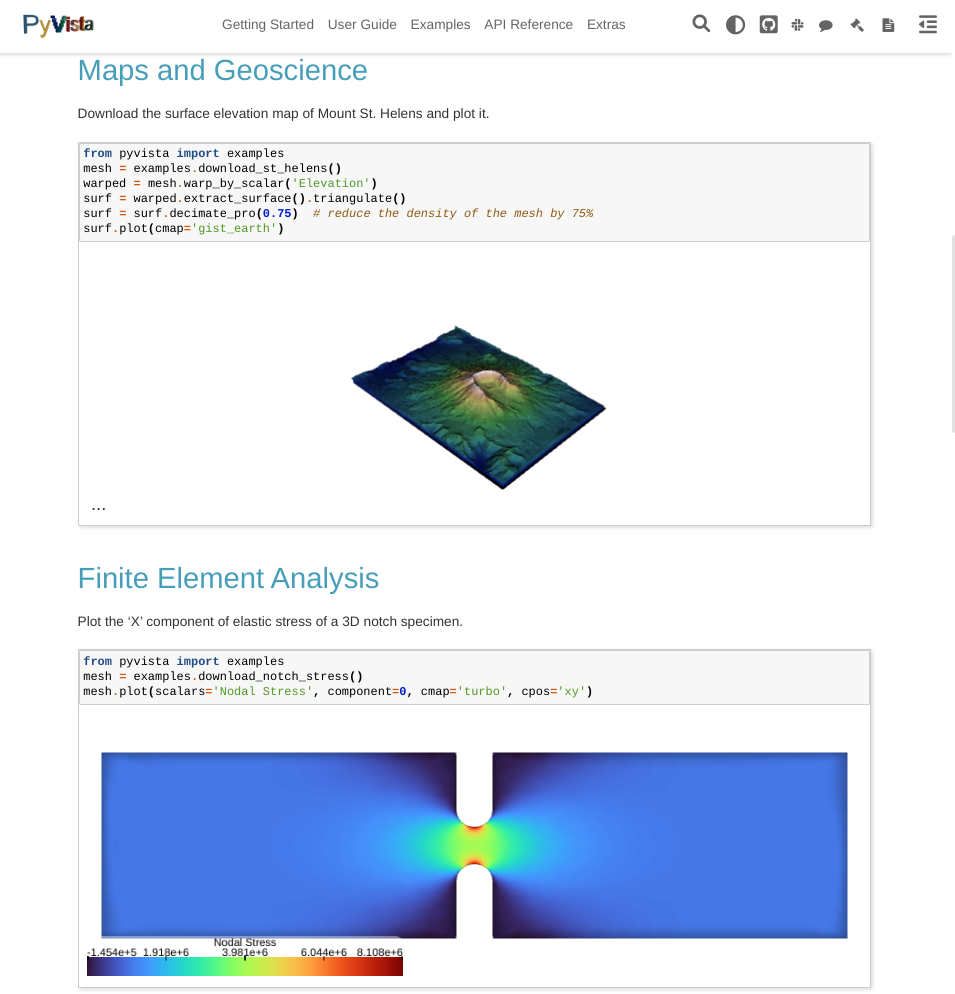
\includegraphics[width=0.9\textwidth]{figures/sphinx.png}}
      \end{column}
    \end{columns}
  \end{center}

\end{frame}


%%%%%%%%%%%%%%%%%%%%%%%%%%%%%%%%%%%%%%%%%%%%%%%%%%%%%%%%%%%%%%%%%%%%%%%%%%%%%%%
\subsection{Tutorial}
\begin{frame}
  \frametitle{Tutorial}

  The \href{https://tutorial.pyvista.org}{PyVista Tutorial} contains a variety of lessons to help you get started with PyVista. The first lessons include:

  \begin{itemize}
  \item Introduction - Using PyVista for 3D Visualization within Python.
  \item Reading and plotting 3D data using the PyVista module and external files.
  \item Learn the basics of the PyVista data types and how to open common 3D file formats to visualize the data in 3D.
  \item Demonstrate many features of the PyVista plotting API to create compelling 3D visualizations and touch on animations.
  \item Demonstrate the PyVista filters API to perform mesh analysis and alteration.
  \end{itemize}

\end{frame}

%%%%%%%%%%%%%%%%%%%%%%%%%%%%%%%%%%%%%%%%%%%%%%%%%%%%%%%%%%%%%%%%%%%%%%%%%%%%%%%
\lastframe{}

\end{document}
